% Options for packages loaded elsewhere
\PassOptionsToPackage{unicode}{hyperref}
\PassOptionsToPackage{hyphens}{url}
%
\documentclass[
]{book}
\usepackage{lmodern}
\usepackage{amssymb,amsmath}
\usepackage{ifxetex,ifluatex}
\ifnum 0\ifxetex 1\fi\ifluatex 1\fi=0 % if pdftex
  \usepackage[T1]{fontenc}
  \usepackage[utf8]{inputenc}
  \usepackage{textcomp} % provide euro and other symbols
\else % if luatex or xetex
  \usepackage{unicode-math}
  \defaultfontfeatures{Scale=MatchLowercase}
  \defaultfontfeatures[\rmfamily]{Ligatures=TeX,Scale=1}
\fi
% Use upquote if available, for straight quotes in verbatim environments
\IfFileExists{upquote.sty}{\usepackage{upquote}}{}
\IfFileExists{microtype.sty}{% use microtype if available
  \usepackage[]{microtype}
  \UseMicrotypeSet[protrusion]{basicmath} % disable protrusion for tt fonts
}{}
\makeatletter
\@ifundefined{KOMAClassName}{% if non-KOMA class
  \IfFileExists{parskip.sty}{%
    \usepackage{parskip}
  }{% else
    \setlength{\parindent}{0pt}
    \setlength{\parskip}{6pt plus 2pt minus 1pt}}
}{% if KOMA class
  \KOMAoptions{parskip=half}}
\makeatother
\usepackage{xcolor}
\IfFileExists{xurl.sty}{\usepackage{xurl}}{} % add URL line breaks if available
\IfFileExists{bookmark.sty}{\usepackage{bookmark}}{\usepackage{hyperref}}
\hypersetup{
  pdftitle={CDL Virtual Advisor (Lab Manual)},
  pdfauthor={Corey Bohil},
  hidelinks,
  pdfcreator={LaTeX via pandoc}}
\urlstyle{same} % disable monospaced font for URLs
\usepackage{color}
\usepackage{fancyvrb}
\newcommand{\VerbBar}{|}
\newcommand{\VERB}{\Verb[commandchars=\\\{\}]}
\DefineVerbatimEnvironment{Highlighting}{Verbatim}{commandchars=\\\{\}}
% Add ',fontsize=\small' for more characters per line
\usepackage{framed}
\definecolor{shadecolor}{RGB}{248,248,248}
\newenvironment{Shaded}{\begin{snugshade}}{\end{snugshade}}
\newcommand{\AlertTok}[1]{\textcolor[rgb]{0.94,0.16,0.16}{#1}}
\newcommand{\AnnotationTok}[1]{\textcolor[rgb]{0.56,0.35,0.01}{\textbf{\textit{#1}}}}
\newcommand{\AttributeTok}[1]{\textcolor[rgb]{0.77,0.63,0.00}{#1}}
\newcommand{\BaseNTok}[1]{\textcolor[rgb]{0.00,0.00,0.81}{#1}}
\newcommand{\BuiltInTok}[1]{#1}
\newcommand{\CharTok}[1]{\textcolor[rgb]{0.31,0.60,0.02}{#1}}
\newcommand{\CommentTok}[1]{\textcolor[rgb]{0.56,0.35,0.01}{\textit{#1}}}
\newcommand{\CommentVarTok}[1]{\textcolor[rgb]{0.56,0.35,0.01}{\textbf{\textit{#1}}}}
\newcommand{\ConstantTok}[1]{\textcolor[rgb]{0.00,0.00,0.00}{#1}}
\newcommand{\ControlFlowTok}[1]{\textcolor[rgb]{0.13,0.29,0.53}{\textbf{#1}}}
\newcommand{\DataTypeTok}[1]{\textcolor[rgb]{0.13,0.29,0.53}{#1}}
\newcommand{\DecValTok}[1]{\textcolor[rgb]{0.00,0.00,0.81}{#1}}
\newcommand{\DocumentationTok}[1]{\textcolor[rgb]{0.56,0.35,0.01}{\textbf{\textit{#1}}}}
\newcommand{\ErrorTok}[1]{\textcolor[rgb]{0.64,0.00,0.00}{\textbf{#1}}}
\newcommand{\ExtensionTok}[1]{#1}
\newcommand{\FloatTok}[1]{\textcolor[rgb]{0.00,0.00,0.81}{#1}}
\newcommand{\FunctionTok}[1]{\textcolor[rgb]{0.00,0.00,0.00}{#1}}
\newcommand{\ImportTok}[1]{#1}
\newcommand{\InformationTok}[1]{\textcolor[rgb]{0.56,0.35,0.01}{\textbf{\textit{#1}}}}
\newcommand{\KeywordTok}[1]{\textcolor[rgb]{0.13,0.29,0.53}{\textbf{#1}}}
\newcommand{\NormalTok}[1]{#1}
\newcommand{\OperatorTok}[1]{\textcolor[rgb]{0.81,0.36,0.00}{\textbf{#1}}}
\newcommand{\OtherTok}[1]{\textcolor[rgb]{0.56,0.35,0.01}{#1}}
\newcommand{\PreprocessorTok}[1]{\textcolor[rgb]{0.56,0.35,0.01}{\textit{#1}}}
\newcommand{\RegionMarkerTok}[1]{#1}
\newcommand{\SpecialCharTok}[1]{\textcolor[rgb]{0.00,0.00,0.00}{#1}}
\newcommand{\SpecialStringTok}[1]{\textcolor[rgb]{0.31,0.60,0.02}{#1}}
\newcommand{\StringTok}[1]{\textcolor[rgb]{0.31,0.60,0.02}{#1}}
\newcommand{\VariableTok}[1]{\textcolor[rgb]{0.00,0.00,0.00}{#1}}
\newcommand{\VerbatimStringTok}[1]{\textcolor[rgb]{0.31,0.60,0.02}{#1}}
\newcommand{\WarningTok}[1]{\textcolor[rgb]{0.56,0.35,0.01}{\textbf{\textit{#1}}}}
\usepackage{longtable,booktabs}
% Correct order of tables after \paragraph or \subparagraph
\usepackage{etoolbox}
\makeatletter
\patchcmd\longtable{\par}{\if@noskipsec\mbox{}\fi\par}{}{}
\makeatother
% Allow footnotes in longtable head/foot
\IfFileExists{footnotehyper.sty}{\usepackage{footnotehyper}}{\usepackage{footnote}}
\makesavenoteenv{longtable}
\usepackage{graphicx,grffile}
\makeatletter
\def\maxwidth{\ifdim\Gin@nat@width>\linewidth\linewidth\else\Gin@nat@width\fi}
\def\maxheight{\ifdim\Gin@nat@height>\textheight\textheight\else\Gin@nat@height\fi}
\makeatother
% Scale images if necessary, so that they will not overflow the page
% margins by default, and it is still possible to overwrite the defaults
% using explicit options in \includegraphics[width, height, ...]{}
\setkeys{Gin}{width=\maxwidth,height=\maxheight,keepaspectratio}
% Set default figure placement to htbp
\makeatletter
\def\fps@figure{htbp}
\makeatother
\setlength{\emergencystretch}{3em} % prevent overfull lines
\providecommand{\tightlist}{%
  \setlength{\itemsep}{0pt}\setlength{\parskip}{0pt}}
\setcounter{secnumdepth}{5}
\usepackage{booktabs}
\usepackage{amsthm}
\makeatletter
\def\thm@space@setup{%
  \thm@preskip=8pt plus 2pt minus 4pt
  \thm@postskip=\thm@preskip
}
\makeatother
\usepackage[]{natbib}
\bibliographystyle{apalike}

\title{CDL Virtual Advisor (Lab Manual)}
\author{Corey Bohil}
\date{2020-05-07}

\begin{document}
\maketitle

{
\setcounter{tocdepth}{1}
\tableofcontents
}
\hypertarget{overview}{%
\chapter{Overview}\label{overview}}

The goal of this book is to serve as a resource for procedures in the lab, tutorials on software and hardware use, and some other advice that I hope will be helpful (e.g., advice on scientific manuscript writing). My guess is that it will serve primarily to get people started in the lab, and also as a refresher on some details about data handling/analyis and use of some equipment.

This is a living document; it will never be ``finished''. We should update it regularly.

This is a \emph{sample} book written in \textbf{Markdown}. You can use anything that Pandoc's Markdown supports, e.g., a math equation \(a^2 + b^2 = c^2\).

The \textbf{bookdown} package can be installed from CRAN or Github:

\begin{Shaded}
\begin{Highlighting}[]
\KeywordTok{install.packages}\NormalTok{(}\StringTok{"bookdown"}\NormalTok{)}
\CommentTok{# or the development version}
\CommentTok{# devtools::install_github("rstudio/bookdown")}
\end{Highlighting}
\end{Shaded}

Remember each Rmd file contains one and only one chapter, and a chapter is defined by the first-level heading \texttt{\#}.

To compile this example to PDF, you need XeLaTeX. You are recommended to install TinyTeX (which includes XeLaTeX): \url{https://yihui.name/tinytex/}.

\hypertarget{getting_started}{%
\chapter{Getting Started in the Lab}\label{getting_started}}

Essential resources and steps

\hypertarget{paperwork}{%
\section{Paperwork}\label{paperwork}}

\hypertarget{software}{%
\section{Software}\label{software}}

You can label chapter and section titles using \texttt{\{\#label\}} after them, e.g., we can reference Chapter \ref{intro}. If you do not manually label them, there will be automatic labels anyway, e.g., Chapter \ref{methods}.

\hypertarget{general-advice}{%
\section{General advice}\label{general-advice}}

\begin{enumerate}
\def\labelenumi{\arabic{enumi}.}
\tightlist
\item
  Don't get attached to any experiment (or theory); just run as many as you can!
\end{enumerate}

\begin{enumerate}
\def\labelenumi{\roman{enumi})}
\tightlist
\item
  Expect to be surprised; your hypotheses will often be wrong.
\item
  We need to publish research, but desperately needing to publish something is a recipe
  for over-interpretation of results
\item
  You can mitigate this to some extent by running lots of studies. Think of it like
  drilling for oil; its good to have a lot of wells going at once.
\end{enumerate}

\hypertarget{essential-reading}{%
\chapter{Essential Reading}\label{essential-reading}}

Here is a list of papers, book chapters, or books that everyone in the lab should read.

\hypertarget{categorization}{%
\section{Categorization}\label{categorization}}

\begin{enumerate}
\def\labelenumi{\arabic{enumi}.}
\setcounter{enumi}{-1}
\tightlist
\item
  Signal detection theory (Swets book chapter; other intro chapters)
\item
  Human Category Learning. Ashby \& Maddox (2005). \url{https://www.annualreviews.org/doi/pdf/10.1146/annurev.psych.56.091103.070217}
\item
  Human Category Learning 2.0. \url{https://www.ncbi.nlm.nih.gov/pmc/articles/PMC3076539/}
\item
  Multidimensional Signal Detection Theory. \url{https://labs.psych.ucsb.edu/ashby/gregory/sites/labs.psych.ucsb.edu.ashby.gregory/files/pubs/ashbysotogrt2015.pdf}
\item
  General recognition theory with individual differences: a new method for examining perceptual and decisional interactions with an application to face perception. \url{https://link.springer.com/article/10.3758\%2Fs13423-014-0661-y}
\item
  Multiple Systems of Perceptual
  Category Learning: Theory and
  Cognitive Tests. \url{https://labs.psych.ucsb.edu/ashby/gregory/sites/labs.psych.ucsb.edu.ashby.gregory/files/pubs/ashbyvalentinhdbkcat_0.pdf}
\item
  The Categorization Experiment:
  Experimental Design and Data Analysis. \url{https://labs.psych.ucsb.edu/ashby/gregory/sites/labs.psych.ucsb.edu.ashby.gregory/files/pubs/ashbyvalentin2018.pdf}
\item
  David Smith prototype v exemplar models
\item
  seminal articles: tversky similarity paper, averaging paper (ashby); medin \& shafer; nosofsky; ashby \& townsend 1986; david smith?
\end{enumerate}

\hypertarget{fnirsneuroimaging}{%
\section{fNIRS/neuroimaging}\label{fnirsneuroimaging}}

\hypertarget{virtualaugmented-reality}{%
\section{Virtual/Augmented Reality}\label{virtualaugmented-reality}}

\hypertarget{statistsical-analysis}{%
\section{Statistsical Analysis}\label{statistsical-analysis}}

\hypertarget{rrmarkdown}{%
\section{R/RMarkdown}\label{rrmarkdown}}

\begin{itemize}
\tightlist
\item
  \href{https://rmd4sci.njtierney.com/}{RMarkdown for Scientists}
\end{itemize}

\hypertarget{productivitygood-research-habits}{%
\section{Productivity/Good Research Habits}\label{productivitygood-research-habits}}

\begin{itemize}
\tightlist
\item
  \href{file:///C:/Users/bohil/Downloads/ResearchHabits.pdf}{Develping good Research Habits}
\item
  especially see the slides labeled ``Reproducability''
\item
  All data edits scripted; all analysis scripted; Graphs \& Tables generated with scripts and automatically pulled into manuscript
\end{itemize}

\hypertarget{intro}{%
\chapter{Data Analysis}\label{intro}}

\hypertarget{github-repositories}{%
\section{GitHub Repositories}\label{github-repositories}}

what to put on github
what NOT to put on github
where to put files - R drive; OneDrive; Google Drive
where to put code - local \& repo
* no data, no output; should be able to regenerate these with 1 click
* folder structure: data; output, code (functions only)
+ sructure of a project
- .rmd files on root directory
- output directory
- code direcotry: R code files containing functions that you call
- all other R code should be right in the rmd file
- SOURCE dependencies (code in R folder) at top of .rmd file that needs them, along with libraries needed for that file.
* how to ignore something: GitIgore (how to add to it: folders; file types, specific files)

\hypertarget{steps-in-every-analysis}{%
\section{Steps in every analysis}\label{steps-in-every-analysis}}

\begin{enumerate}
\def\labelenumi{\arabic{enumi})}
\item
  Read in data, get into Tidy format
\item
  Manipulate data as needed
\item
  Visualize data
\end{enumerate}

use ggplot2 package

Always do this before any statistical analysis. Look at the data to see what is going on. After that you can do statistical analysis (e.g., ANOVA/regression, t-tests, etc.) to see if any obsered differences are large enough to be considered reliable (i.e., ``statistically significant'').

You should have plots summarizing each of your variables, as well as combinations of variables that are obviously of importance (e.g., block x accuracy)

Types of plots for variable types:
- 2 continuous variables (e.g., age, height): scatterplot (GGPLOT); line (GGPLOT)
etc\ldots{}

\begin{enumerate}
\def\labelenumi{\arabic{enumi})}
\setcounter{enumi}{3}
\tightlist
\item
  Statistical analysis
\end{enumerate}

\begin{quote}
\begin{quote}
data analysis
1) - scale types: ALWAYS consider first!
metric, ordinal, etc
need to know this for plotting and statistical analysis
2) - long form vs wide form data; transforming between these
important for plotting, ANOVA,
2.5) data assumption: normally distributed? y = data; completely unknown; normal? tests
3) general linear model
correlation; simple regression, multiple regression
\textgreater{} prediction- yes! causation - no!
\textgreater{} causation - need experiment (control timing of cause(s)!! (only way w obs data = SEM/BAYES NETS)
ttest logic
anova logic
ANOVA is a special case of regression with dichotomos predictors! (same mathematical model)
what is the linear model doing? linear equation + normally distributed noise
\textgreater{} assumption of the model - normally distributed data ==\textgreater{} the NOISE!! (unexplained variance part).
\end{quote}
\end{quote}

how do do anovas/regression w software
\textgreater\textgreater{} spss
\textgreater\textgreater{} jasp
\textgreater\textgreater{} R

how to interpret \& report results (APA style; what to report; how to INTERPRET!)
\textgreater\textgreater{} ANOVA
\textgreater\textgreater{} regression?

\begin{quote}
what if assumptions are violated?
\textgreater{} nonparametric statistical tests (robust to violations)
\end{quote}

frequentist (classical) vs bayesian statistics
\textgreater\textgreater{} why? replicability!
\textgreater\textgreater{} problems w classical (multiple comparisons; null hypothesis not what we want, no peeking/cheating!)
\textgreater\textgreater{} problems solved by bayesian
\textgreater\textgreater{} is NHST/classical worthless? NO!! its just that bayesian seems to be BETTER (more reliable by avoiding some of the problems that reduce reliability in terms of reproducability (replicability)
\textgreater{} statistics is about REPLICATILBITY
\textgreater{} replicability is about what is true!\\
\textgreater{} we want to avoid publishig things that are not true! we want us (and others) to be able to replcate; bayesian may help us play it safer

so what do we do in stats? 2 things
1) estimation (e.g., mean, variance, difference between groups, learning rate, regreession coefficient)
2) inference (e.g., difference between groups? effect of treatement? theory/model 1 better than theory/model 2?)
note: both classical and bayesian apply the SAME MODEL!! GENERAL LINEAR MODEL
\textgreater\textgreater{} they differ in terms of how they ESTIAMTE the parameters of the model(s)
\textgreater\textgreater{} they differ in how we INTERPET THE RESULTS (i.e., make infernces from the data!)

\begin{enumerate}
\def\labelenumi{\arabic{enumi})}
\setcounter{enumi}{4}
\tightlist
\item
  Data modeling
\end{enumerate}

You can label chapter and section titles using \texttt{\{\#label\}} after them, e.g., we can reference Chapter \ref{intro}. If you do not manually label them, there will be automatic labels anyway, e.g., Chapter \ref{methods}.

Figures and tables with captions will be placed in \texttt{figure} and \texttt{table} environments, respectively.

\begin{Shaded}
\begin{Highlighting}[]
\KeywordTok{par}\NormalTok{(}\DataTypeTok{mar =} \KeywordTok{c}\NormalTok{(}\DecValTok{4}\NormalTok{, }\DecValTok{4}\NormalTok{, }\FloatTok{.1}\NormalTok{, }\FloatTok{.1}\NormalTok{))}
\KeywordTok{plot}\NormalTok{(pressure, }\DataTypeTok{type =} \StringTok{'b'}\NormalTok{, }\DataTypeTok{pch =} \DecValTok{19}\NormalTok{)}
\end{Highlighting}
\end{Shaded}

\begin{figure}

{\centering 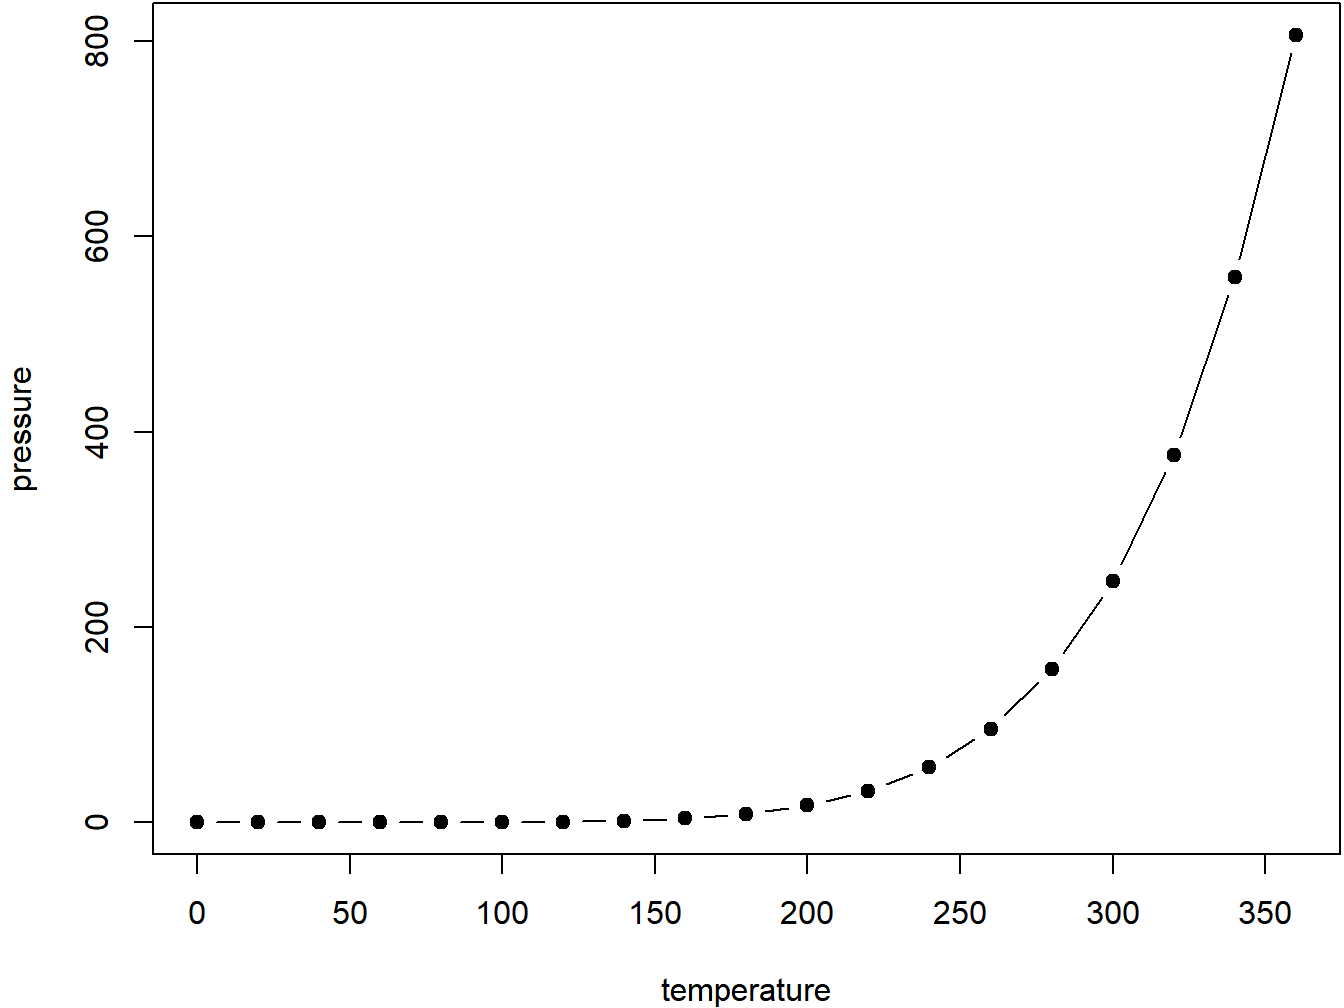
\includegraphics[width=0.8\linewidth]{bookdown-demo_files/figure-latex/nice-fig-1} 

}

\caption{Here is a nice figure!}\label{fig:nice-fig}
\end{figure}

Reference a figure by its code chunk label with the \texttt{fig:} prefix, e.g., see Figure \ref{fig:nice-fig}. Similarly, you can reference tables generated from \texttt{knitr::kable()}, e.g., see Table \ref{tab:nice-tab}.

\begin{Shaded}
\begin{Highlighting}[]
\NormalTok{knitr}\OperatorTok{::}\KeywordTok{kable}\NormalTok{(}
  \KeywordTok{head}\NormalTok{(iris, }\DecValTok{20}\NormalTok{), }\DataTypeTok{caption =} \StringTok{'Here is a nice table!'}\NormalTok{,}
  \DataTypeTok{booktabs =} \OtherTok{TRUE}
\NormalTok{)}
\end{Highlighting}
\end{Shaded}

\begin{table}

\caption{\label{tab:nice-tab}Here is a nice table!}
\centering
\begin{tabular}[t]{rrrrl}
\toprule
Sepal.Length & Sepal.Width & Petal.Length & Petal.Width & Species\\
\midrule
5.1 & 3.5 & 1.4 & 0.2 & setosa\\
4.9 & 3.0 & 1.4 & 0.2 & setosa\\
4.7 & 3.2 & 1.3 & 0.2 & setosa\\
4.6 & 3.1 & 1.5 & 0.2 & setosa\\
5.0 & 3.6 & 1.4 & 0.2 & setosa\\
\addlinespace
5.4 & 3.9 & 1.7 & 0.4 & setosa\\
4.6 & 3.4 & 1.4 & 0.3 & setosa\\
5.0 & 3.4 & 1.5 & 0.2 & setosa\\
4.4 & 2.9 & 1.4 & 0.2 & setosa\\
4.9 & 3.1 & 1.5 & 0.1 & setosa\\
\addlinespace
5.4 & 3.7 & 1.5 & 0.2 & setosa\\
4.8 & 3.4 & 1.6 & 0.2 & setosa\\
4.8 & 3.0 & 1.4 & 0.1 & setosa\\
4.3 & 3.0 & 1.1 & 0.1 & setosa\\
5.8 & 4.0 & 1.2 & 0.2 & setosa\\
\addlinespace
5.7 & 4.4 & 1.5 & 0.4 & setosa\\
5.4 & 3.9 & 1.3 & 0.4 & setosa\\
5.1 & 3.5 & 1.4 & 0.3 & setosa\\
5.7 & 3.8 & 1.7 & 0.3 & setosa\\
5.1 & 3.8 & 1.5 & 0.3 & setosa\\
\bottomrule
\end{tabular}
\end{table}

You can write citations, too. For example, we are using the \textbf{bookdown} package \citep{R-bookdown} in this sample book, which was built on top of R Markdown and \textbf{knitr} \citep{xie2015}.

\hypertarget{writing}{%
\chapter{Writing}\label{writing}}

Some guidelines and advice on scientific writing.

\hypertarget{general-advice-1}{%
\section{General advice}\label{general-advice-1}}

Use R Markdown
* spell checking in .Rmd
* Creating a bibliography using .bib files

\hypertarget{start-writing-early}{%
\section{Start writing early}\label{start-writing-early}}

Write a short outline/draft of the method section when planning an experiment
* as you add details, add this to the outline (can be bullet points at first).
* IMPORTANT: If/When the experiment becomes a reality, write out the complete detailed Method Section right away - don't wait until after data collection is done and data is analyzed. You will remember why things were done better if you write it immediately. Also power analysis should be done for every study and reported here right from the start.

\begin{itemize}
\item
  Introduction/Lit review - same as for methods. Work through the logic of your arguments and enumerate them, and their rationale(s) in an intro section BEFORE you run a study. You can wait to turn this into prose as soon as the experiment becomes a reality (i.e., is running), but then you should write up a draft of the intro/lit review/experiment overview/hypotheses sections and any needed theoretical sections (e.g., plan for statistical analysis of fNIRS data, General Recognition Theory section, etc.).
\item
  You can also put in a lot of the references at this time, and make sure your reference section is building correctly as you go!
\item
  Summarize all PLANNED analyses and write as much of this as you can ahead of time too. This will be more tentative in terms of the writing, but the analysis itself should be completely knowable before starting the experiment.\\
  In fact - your study variables imply what analyses you'll carry out (e.g., what the variables are, the scale of the data will dictate the statistical analyses, modeling analysis planned, ANOVA details)
\end{itemize}

\hypertarget{misc}{%
\subsection{misc}\label{misc}}

\begin{itemize}
\item
  every study can be boiled down to a single page summary of results; we should always create this before writing
\item
  only write after the story is clear - the results are analyzed and evaluated and we've based our conclusions on them in the summary; then write the prose
\item
  list: honors thesis topics we'd like to see (will consider supervising these only)
\end{itemize}

on motivation, time, \& energy
\textgreater{} most important thing will also get the least external motivation -- research/writing
\textgreater\textgreater{} find a time to do this regulary; eg., 9-noon every weekday. no distractions! (phone, email, people).
everythign else you have to do WILL get done, because it HAS TO (nonstop external pressure to complete things): TA duties; class requirements; program requirements; talks/posters
\textgreater{} this is the most insidious threat to your success. if you establish only 1 good habit let it be this: set aside time every day that is for research (whatever phase of the project you are at). that's 15 hours/week. i suggest 1st thing every morning to get it done. then you can do other things with your day and relieves some pressure
\textgreater{} try not to make your problems other peopl'es problems: i.e., if yoiu have a big assigment, let your advisor know, but get in the habit of just planing ahead to avoid letting it disrupt your responsibilities to the lab for research.
\textgreater\textgreater{} image: you can lead a horse to water but you can't make him drink
\textgreater\textgreater{} even i struggle with this advice from time to time, but it has worked far better for me than anything else over the years
? do you want to know the secret to success in academics? that's it. i just told it to you. not that glamorous huh? but will you take this advice to heart and establish this habit? only you can decide. the biggest killers of productivity (and therefore success in academe) is distraction, time management, and dealing with stress. establishing this habit addresses them all at once. its the best advice i can give you. (horse/water) make this an iron rule, and you will thrive.
- another piece of advice has to do with energy/motivation (follow your energy) but that is another matter and is somewhat complicated by the constraints of working in your advisor's lab, where projects need to get completed.

\begin{itemize}
\tightlist
\item
  projects/ideas
  \textgreater{} venn diagram models
  \textgreater{} year 1: they are a complete subset
  \textgreater{} year 4: overlapping subsets
  \textgreater{} never: separate circles
  \textgreater\textgreater{} authorship: using lab resources which i'm ultimately responsible for (this includes my time and effort in advisement); i'm not in favor of you doing something on your own without an advisor; if you want to work on a project with a different advisor, it needs my approval first. look at it from my perspective: trying to run this lab, need people who want to learn from me. if you decide this is not for you, let me know - maybe there's a different advisor. best not to go to them first. if youre not comfortable talking to me about this, talk to the program director (or above if i'm somehow the director at some point)
  \textgreater{} authorship: i'll almost always be corresponding author; maybe not when you're at end of training.
\end{itemize}

\hypertarget{functional-near-infrared-spectroscopy-fnirs}{%
\chapter{Functional Near-Infrared Spectroscopy (fNIRS)}\label{functional-near-infrared-spectroscopy-fnirs}}

\hypertarget{nirsport-88-system-nirx-medical-technologies-inc.}{%
\section{NIRSPort 88 system (NIRX Medical Technologies, Inc.)}\label{nirsport-88-system-nirx-medical-technologies-inc.}}

We have a NIRX nirsport88 mobile system, which no longer appears on the Nirx website.

Nevertheless, everything needed (data acquisition \& analysis software, support, training) can be found on the NIRx website:
\url{https://nirx.net/}

\begin{enumerate}
\def\labelenumi{\arabic{enumi}.}
\tightlist
\item
  download analysis software \& and read manual
\end{enumerate}

\begin{itemize}
\tightlist
\item
  \url{https://nirx.net/software}
\item
  \url{https://nirx.net/nirslab-1}
\item
  NITRC site (where you'll actually download): \url{https://www.nitrc.org/frs/?group_id=651}
\end{itemize}

As you read the manual, try it out with real data (e.g., nirx.net has some data sets you can download if needed).

\begin{enumerate}
\def\labelenumi{\arabic{enumi}.}
\setcounter{enumi}{1}
\tightlist
\item
  read this document on cortical functions for background on localizing Brodmann areas we'll be recording from using the International 10-20 system used in EEG
\end{enumerate}

\begin{itemize}
\tightlist
\item
  \url{https://thebrainstimulator.net/docs/external/Trans_Cranial_Technologies-cortical_functions_ref_v1_0.pdf}
\end{itemize}

Also very helpful: Wikipedia page on Brodmann areas (w. hyperlinks to each area):
\url{https://en.wikipedia.org/wiki/Brodmann_area}
- Provides summary of functions along with references for each brodmann area, and usually an image showing the region

TO ADD:
1. need note on how to examine probe layouts in nirslab

\hypertarget{fnir-devices-imager-1000-from-fnir-devicesbiopac}{%
\section{fNIR Devices Imager 1000 (from fNIR Devices/Biopac)}\label{fnir-devices-imager-1000-from-fnir-devicesbiopac}}

\hypertarget{virtual-augmented-reality}{%
\chapter{Virtual \& Augmented Reality}\label{virtual-augmented-reality}}

In the lab we have the following equipment\ldots{}

\hypertarget{virtual-reality}{%
\section{Virtual Reality}\label{virtual-reality}}

\hypertarget{augmented-reality}{%
\section{Augmented Reality}\label{augmented-reality}}

\hypertarget{program-requirements}{%
\chapter{Program Requirements}\label{program-requirements}}

Milestones for the UCF Human Factors \& Cognitive Psychology Program (for graduate students)

\hypertarget{undergraduate-research-assistants}{%
\section{Undergraduate research assistants}\label{undergraduate-research-assistants}}

\hypertarget{volunteer-form}{%
\subsection{Volunteer form}\label{volunteer-form}}

\begin{enumerate}
\def\labelenumi{\arabic{enumi}.}
\tightlist
\item
  Volunteer form
\end{enumerate}

\begin{itemize}
\tightlist
\item
  Before an individual can start his or her volunteer assignment, the departments must complete the Volunteer Services Agreement. Go here for details and to access the form(s):
\end{itemize}

\url{https://compliance.ucf.edu/enterprise-risk-management/university-volunteers/}

\begin{enumerate}
\def\labelenumi{\arabic{enumi}.}
\setcounter{enumi}{1}
\tightlist
\item
  If you want your voluneering to appear on your transcript, you must submit a URA form.
\end{enumerate}

\begin{itemize}
\tightlist
\item
  We need to ask the undergraduate advising office for this form
\item
  From Director of Undergraduate Advising Karen Cox: ``The process is departmentally driven. So, the Advising Center helps with the admin side of things for the faculty. To make it easier for you.''
\end{itemize}

``You are welcome to tell students to send the forms to \href{mailto:psychadvising@ucf.edu}{\nolinkurl{psychadvising@ucf.edu}} after they have your approval, fill out their student info, fill in the assignments, and your signature is on the form.''

So it appears you need to e-mail the advising office for the form and attempt to fill it out. Dr.~Bohil can then approve it before you submit it.

\begin{itemize}
\tightlist
\item
  point of contact: Karen Cox, Director of Undergraduate Advising: \url{https://sciences.ucf.edu/psychology/people/kox-karen/}
\end{itemize}

  \bibliography{book.bib,packages.bib}

\end{document}
